\begin{comment}
\end{comment}

\section{Exemple de graphique}

La figure~\ref{fig:phdcomics} est très drôle, sérieusement.

\begin{figure}[htb]
    \begin{center}
        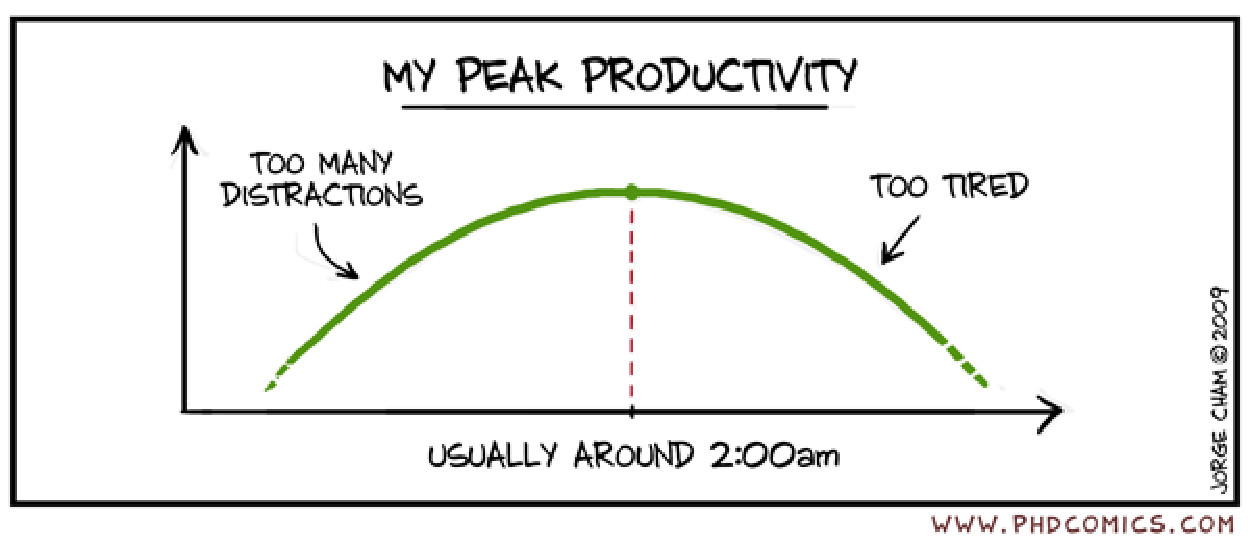
\includegraphics[width=0.8\columnwidth]{Figures/phd083109s.pdf} 
        \caption{Figure à la fois hilarante et véridique.}
        \label{fig:phdcomics}
        \vspace{-10pt}
        \caption*{ Image tirée du webcomic "Piled Higher and Deeper" par Jorge Cham
                   \href{www.phdcomics.com}{www.phdcomics.com}. 
                   Ce long caption ne sera pas dans la table des figures.
                 }
    \end{center}
\end{figure}

\section{Remplissage}
\kant[11-14]
